Calculating the path delays and angles from labeled points was not done within the time constraints of the course, which inspired this new approach. Specifically, the problem was translating the (x,y) coordinates to the correct path angle and delay. As a work around the authors tried using a DNN to go directly from the images to the path components, completely skipping the object detection, coordinate translation, and path calculations. In essence, the idea was to brute force a solution using DNN. The model built was an image regression model, taking each of the generated images and trying to predict the path gains and delays. Some modifications had to be made, for instance the path components had to be normalized since they all had different scales. Additionally, the paths had to be sorted in the output, so the model knew which paths corresponded to the brightest points. Since it is known the path information is encoded in the image, the theory is that the right DNN would be able to extract it and calculate the path components. However, this effort was in vain, as the DNN did not predict the paths with enough accuracy. When the DNN was unable to solve the problem it was simplified to show a proof of concept. The noise was removed from the channel and the number of paths was set to be constant. 

The model was built using Autokeras, which is a DNN framework that uses Keras from Tensorflow. Autokeras is a tool to automatically generate and validate Keras models. The library treats the depth and width of the DNN's hidden layers as a hyper-parameter and optimizes the DNN structure accordingly. Initially, the models were trained locally, configured to run on a 4GB GTX1650 with Tensorflow 2.4, CUDA 11.0 and CuDNN 8.4. Despite the efforts to configure Tensorflow to train on the GPU, this still proved to be quite slow for training and testing many DNNs with a large data set. To reduce the training time the ML was moved to Google Colab; which offered a free virtual machine with a good GPU. Often Colab provided a 16GB Tesla V100 GPU. There were some limitations with Colab such as the session time and virtual storage. Autokeras stores many DNN while training with many different checkpoint versions. This quickly filled the storage on colab, limiting the amount of data used to train the network. Additionally, the Colab session would timeout and the data stored locally would be lost. 

The first model was trained using 5000 different simulated channels, with 5 different DNN's tested with a maximum epoch count of 1000. The training process took 20 hours running on Google Colab. The best model of the 5 barely predicted values better then random. The data was normalized to be in the range of 0 to 1, using a 'min\_max\_scalar' from sklearn. The model was trained to predict the path angles and delays. The resulting RMSE was 0.3, which was not much better then predicting random values. Figure \ref{fig:dnnres} shows the predicted values plotted against the true values for the path delays and angles of the first path.
\begin{figure}[H]
    \subfigure[]{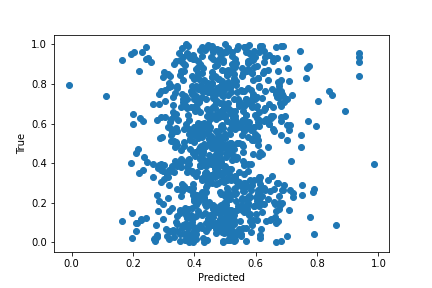
\includegraphics[width=0.45\textwidth]{T_1.png}} 
    \subfigure[]{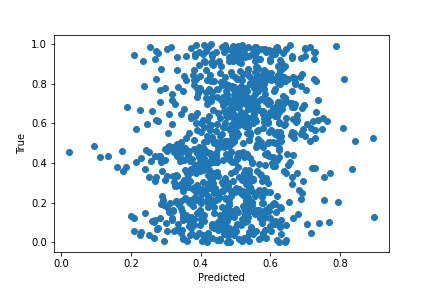
\includegraphics[width=0.45\textwidth]{AoA_1.png}}
    \caption{Predicted vs True Values for Path 1's (a) Delay (b) Angle}
    \label{fig:dnnres}
\end{figure}
\noindent
It is clear when looking at these results the predictions are all normally distributed around the mean and do not correlate with the true values. The better the predicted values, the closer they would be to the \(y=x\) line.

The first attempt seemed fundamentally flawed, too much time was spent training the model and not enough resources were focused on identifying the correct DNN. The second attempt used drastically less data, but tested far more DNNs. The data set consisted of 500 channel images and Autokeras trained 30 models over 100 epochs. Reviewing the results of the previous attempt the validation error was improved by an order of magnitude over epoch 101-1000. The extra hours spent training were not useful since the model did not generalize. This attempt was significantly faster, only running for 6 hours however came with a new issue. The 30 DNNs trained generated a massive amount of data to be stored (60GB+), which exceeded the storage capacity on the colab instance. This caused the virtual machine to crash, with the model unrecoverable. 

Instead of running on the server this approach was tested locally, and showed promising results. The local GPU could not support this heavy of a model, so the images were scaled down to 128 pixels\(^{2}\) from 384 pixels\(^2\); reducing the number of input nodes in the network by an order of magnitude. This increased the size of training batches significantly, reducing the training time for each epoch to tens of seconds instead of a full minute. This comes at a cost though, the resolution of the image is directly related to the accuracy of our predictions. Additionally, only the path delays were predicted to further reduce the complexity. Even with the simplification it took 10 hours to generate and train the models locally with the GTX 1650. The resulting model had a RMSE of 0.1, outperforming the previous attempt by a factor of 3; however, it was not enough to accurately reconstruct the channel. This shows the DNN architecture from this approach is far better for solving the problem then the one generated in the first approach. Figure \ref{fig:laptopT} shows the predicted vs true results for the first path. It does not look drastically better then the previous plots, however, the density around the $y=x$ is much higher, as shown by the improved RMSE. Although, had the DNN architecture generated from this approach been trained with 1000 epochs, full image resolution, and the 5000 image data set used for the previous trial, it would likely improve performance dramatically. This was be the next step for the DNN approach, however due to the massive amount of time to test these models it was not completed in time for the report submission.

\begin{figure}[H]
    \centering
    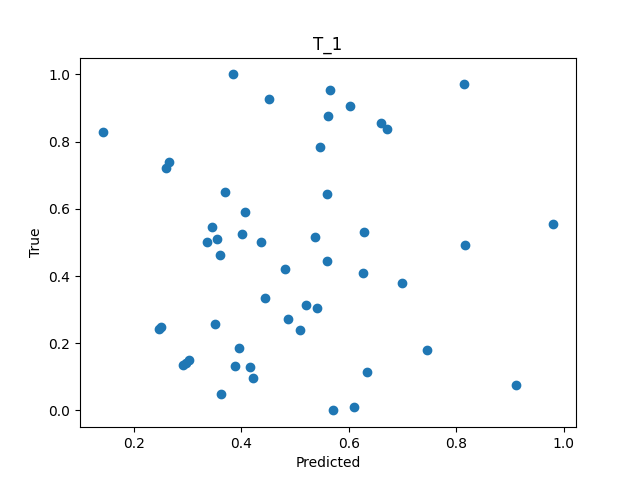
\includegraphics[width=0.49\textwidth]{figures/T_1_laptop.png}
    \caption{Laptop Predictions with Drastically Less Resources}
    \label{fig:laptopT}
\end{figure}
